\chapter{Optimization Strategies}
\label{ch:optimization}

The following chapter will present optimization strategies which were used to
accelerate the mean shift image segmentation. The presented strategies are not
only valid for \gls{CUDA}, they can be applied to many parallel machines which
are build after the shared memory or \gls{SPMD} model. The chapter is divided in
several sections. Each section will present an optimization. The are major and
minor optimization that are examined where mostly major optimization give higher
speedup whereas minor optimization give lower speedup. 

Many of the optimization are hardware centric, which means that one has to have
a good knowledge about the architecture to understand which steps can be
undertaken to accelerate the algorithm and which where even possible. Each
section will cover the architectural specialty which led to perform the specific
optimization. The first optimization of the next section is a general rule when
trying to accelerate an algorithm, offload compute intensive parts. The succeeding
sections respectively optimizations are in chronological order and where applied
in that order, identifiable by the ever increasing speedups. 


\section{Test \textit{\&} Benchmark Configuration} % (fold)
\label{sec:test__benchmark_configuration}
For measuring the run-time the \gls{CUDA} timers are used. They have a
resolution of approximately half a microsecond. The timings are measured on the
\gls{GPU}, and hence they are operating system independent. Further benchmark
metrics like bandwidth, coalesced or uncoalesced access to global,shared and
local memory or time spent in device functions were reported by cudaprof a
profiler for \gls{CUDA} programs. OProfile was used on the host side for
profiling the program.

For the measurement a image with a dimension of 256$\times$256 pixel was used
and with the following parameters: \textsf{sigmaS} = 7, \textsf{sigmaR} = 6.5
and \textsf{minRegion} = 20 (\textsf{minRegion} is used for pruning regions
smaller than 20 pixel).
% section test_\&_benchmark_configuration (end)


\section{Offload Compute Intensive Parts}
\label{sec:offload_intensive}
\fpAdd{\timegold}{0,0}{9616,77}
\fpAdd{\timecuda}{0,0}{1942}
\fpDiv{\speedup}{11310}{1942}

As shown in \autoref{ch:algorithm_analysis} {\color{red} DESIGN IMPLEMNtAtION..}
the most compute intensive part of the mean shift segmentation is the filtering
step. bla bla blbub.. mal sehen was vorne noch steht 98\%. In this case the most
compute intensive part is 98.2\% of the complete run-time and hence a valuable
part to offload. All other parts have no significant part of the run-time but
when optimizing it can happen that these other part grow in terms of run-time
and the before most compute intensive part with a very high percentage drops to
a low percentage and hence the percentages of all other parts increase and
become very compute intensive. 

In other cases the run-time is often distributed among several parts and in this
case it should be tried to offload as much as possible of the computational parts
to an accelerator as the \gls{GPU}. In the first place the focus will be on the
filter part that is executing in total 99.1\% of the run-time.

For the following considerations about speedup the \autoref{eq:speedup} will be
used to calculate the speedup. 

In {\color{red} bezug zu design implementierun} it was shown how to design and
to implement the algorithm to offload the important parts to the \gls{GPU} and
the first naive implementation of the mean shift filter in \gls{CUDA} resulted
in a speedup of

\begin{equation*}\label{eq:speedup0}
	S = \frac{T_{CPU}}{T_{GPU}} = %
	\frac{\unit[\timegold]{ms}}{\unit[\timecuda]{ms}} = \speedup
\end{equation*}

times faster than the \gls{CPU} version. The reference time was generated from
\href{http://www.caip.rutgers.edu/riul/research/code.html}{ \gls{EDISON}}. It
reports timings for filtering and segmentation.
The first implementation was just a naive implementation without regarding the
hardware restrictions and without exhausting the hardware potential. In
\autoref{sec:data_flow} it was shown that in every iteration of calculating the
mean shift vector the algorithm fetches color values for every pixel contained
in the search window. The search window is defined by \textsf{sigmaS} the
spatial window and \textsf{sigmaR} the range window. For now, only
\textsf{sigmaS} is important since that value spans the spatial window over
the pixel (see \autoref{lst:msk}). 



\section*{Global Memory \textit{\&} Coalescing} 
\label{sec:coalescing}

One important fact for coalescing is the sequential accesses to global memory
should be grouped together. A simple optimization is to use the \emph{float4}
data type available in \gls{CUDA}. After rewriting the algorithm the new speedup
was 
\fpAdd{\timecuda}{0,0}{1464}
\fpDiv{\speedup}{\timegold}{\timecuda}
\begin{equation*}\label{eq:speedup1}
	S = \timegold\ ms/\timecuda\ ms = \speedup
\end{equation*}

basin of attraction, random access to global memory, not knowing where each pixel
is moving to. Switching to \emph{textures} (glossary texturess) yield to a huge
speedup of 

\fpAdd{\timecuda}{0,0}{260}
\fpDiv{\speedup}{\timegold}{\timecuda}
\begin{equation*}\label{eq:speedup2}
	S = \timegold\ ms/\timecuda\ ms = \speedup
\end{equation*}


\section*{Division Instruction Optimization}
\label{sec:expensive_divisions}
Every hardware instruction is taking a specific amount of clock cycles to complete. 
For single-precision floating-point arithmetic instructions like add, multiply
or multiply-add take 4 clock cycle to complete. Whereas the single-precision
floating-point division takes about 36 clock cycles, which is 9$\times$ slower 
than the common arithmetic instructions. Therefore divisions should be avoided
as much as possible to increase instruction throughput. 


Having a look at \autoref{alg:msf} it can be seen that in the calculation of the
mean shift vector divisions occur. The denominator is the size of the search
window. In this implementation the size of the search window is not changing and
hence a constant. This circumstance can be exploited and the reciprocal can be
calculated. The reciprocal can then be substituted by the division and denominator
to produce faster multiplications.

For example if it looks like this
\begin{lstlisting}[caption=Expensive divison, label=lst:division]
//Determine if inside search window
//Calculate distance squared of sub-space s
float dl = (luv.x - yj_2) / sigmaR;               
float du = (luv.y - yj_3) / sigmaR;               
float dv = (luv.z - yj_4) / sigmaR;
\end{lstlisting}
one can calculate \textsf{rsigmaR} = 1.0f/\textsf{sigmfaR} in advance and everywhere where a
division by \textsf{sigmaR} occurs replace it into a multiplication. The
resulting code is then
\begin{lstlisting}[caption=Division turned into fast multiplication, label=lst:precalcdivision]
//Determine if inside search window
//Calculate distance squared of sub-space s
float dl = (luv.x - yj_2) * rsigmaR;               
float du = (luv.y - yj_3) * rsigmaR;               
float dv = (luv.z - yj_4) * rsigmaR;
\end{lstlisting}

With this technique the kernel code is free of divisions except only one that
cannot be eliminated since the value is changing throughout the calculations.
This optimization yielded a speedup of

\fpAdd{\timecuda}{0,0}{203}
\fpDiv{\speedup}{\timegold}{\timecuda}
\begin{equation*}\label{eq:speedup3}
	S = \frac{\unit[\timegold]{ms}}{\unit[\timecuda]{ms}} = \speedup
\end{equation*}


\section{Run Configurations} % (fold)
\label{sec:run_configurations}

It is important to check the best run configuration. Each run configruation 
has its benefit. Some can exploit the bandwidth to the global memory some can
benefit from the cache of the texture. Furthermore it is important to keep the
hardware busy to hide memory latencies. Busy means that one should to design 
the application to use threads and blocks so that the hardware can balance the 
work across the multiprocessors. 

After testing all configurations the 
best fit was a $8x32=256 threads$ configuration.

\fpAdd{\timecuda}{0,0}{181}
\fpDiv{\speedup}{\timegold}{\timecuda}
\begin{equation*}\label{eq:speedup4}
	S = \timegold\ ms/\timecuda\ ms = \speedup
\end{equation*}


% section run_configurations (end)

\section{Use the Float Data Type where Ever Possible}
The \gls{CUDA} Programming Guide \citep{citeulike:3325943} highly recommends the
use of the \emph{float} type for single-precision floating-point code.
Additionally it is recommended to use the single-precision floating-point
mathematical functions. One should use the $float$ data type where ever
possible. The \glspl{GPU} are highly optimized for floating point calculations.
After converting all integer calculations to floating point operations another
speedup was achieved.
\fpAdd{\timecuda}{0,0}{175}
\fpDiv{\speedup}{\timegold}{\timecuda}
\begin{equation*}\label{eq:speedup5}
	S = \frac{\unit[\timegold]{ms}}{\unit[\timecuda]{ms}} = \speedup
\end{equation*}
On current \gls{GPU} hardware integer operations can be very expensive in terms
of clock cycles. The situation can change with future \gls{GPU} architecture check
against \emph{Fermi} the new architecture from {\slcsmallcaps{NVIDIA}} 
{\color{red}{\autoref{sec:fermi}}}.



\section{Avoid Branch Divergence} % (fold)
\label{sec:avoid_branch_divergence}
On a architecture with such high throughput of calculations per cycle it is preferred
to calculate values rather then generating them through $if$ and $else$ statements.
The remaining $if$ and $else$ statements where arranged in such a way so that a 
thread is exiting early from the loop and avoiding uneccesary calculations. This leads
of course to higher branch divergence but the execution time is lower. 
\fpAdd{\timecuda}{0,0}{125}
\fpDiv{\speedup}{\timegold}{\timecuda}
\begin{equation*}\label{eq:speedup6}
	S = \timegold\ ms/\timecuda\ ms = \speedup
\end{equation*}

\section{Shared Memory} % (fold)
\label{sec:shared_memory}
The optimization guides state that one should use shared memory to avoid 
redundant transfers from global memory. But in this case the accesses are not 
known in advance and would lead to heavy reduce in run time as the access to 
shared memory from the threads would lead to many bank conflicts. 

\section{Know the Algorithm} % (fold)
\label{sec:know_the_algo}
This section is not related to the hardware more related to the software part of 
the algorithm. After all the other optimizations done it was obvious that there
was not more room for many optimizations that target the hardware. The focus went
on to the algorithm and its peculiarity when filtering the image. 

The idea was to examine how many iterations in average the algorithm needs to
filter the image. In the original code of \gls{EDISON} there is variable named
\textsf{iterationCount} which limits the iteration count to 100 per pixel. The
comment in the source code says \textit{``Iteration count is for speed up
purposes only -- it does not have any theoretical importance"} that brought up a
question, why it is needed anyway when the mean shift algorithm converges
\citep{citeulike:462300}. For this the source code was modified in that way
that for each pixel the iteration count was reported. A precise look a the 
generated numbers showed that some pixel have iteration counts of 100. 

To have an clue if its worth to continue the research into this direction several
tests were done. Looking at the iteration count it sticks out that most of the 
pixel are finished after about 10 iterations, it was strange to see that several
pixel were iterating till 100. 

The approach taken was to limit the iteration count not to 100 but to 10 and 50.
Setting the limit to 10 and executing the \gls{CPU} and \gls{GPU} version the
speedup was 
 
\fpAdd{\tgold}{0}{7369}
\fpAdd{\tcuda}{0}{29}
\fpDiv{\speedup}{\tgold}{\tcuda}
\begin{equation*}\label{eq:speedup7}
		S = \frac{\unit[\tgold]{ms}}{\unit[\tcuda]{ms}} = \speedup
\end{equation*}

Setting the limit to 50 and executing the \gls{CPU} and \gls{GPU} version again
the speedup was
\fpAdd{\tgold}{0}{10373}
\fpAdd{\tcuda}{0}{82}
\fpDiv{\speedup}{\tgold}{\tcuda}
\begin{equation*}\label{eq:speedup8}
	S = \frac{\unit[\tgold]{ms}}{\unit[\tcuda]{ms}} = \speedup
\end{equation*}

In the case where the limit is 10 the \gls{GPU} could achieve a speedup of 
\fpDiv{\speedup}{\tgold}{\tcuda} \speedup$\times$ because all multiprocessors
are busy then and are not idle as in the case when the limit is 100 and just a few
threads are calculating and the rest idles. The algorithm is as fast as the slowest
thread which is iterating until 100. 

A candidate with iteration count of 100 is picked up from the iteration list and
examined further. For this the magnitude squared (the length) of the mean shift
vector is analyzed over the iterations. When the mean shift vector approaches
the convergence point the magnitude becomes smaller and smaller until it falls
under a small number. In this implementation this small number is
$\epsilon=0.01$. Then it can be said that the mean shift vector has reached the
basin of attraction.

\begin{lstlisting}[caption=Magnitude squared of pixel 10992, label=lst:msp]
10992 - 0.00000 - 1
10992 - 2.52029 - 2
10992 - 2.52029 - 3
10992 - 2.52029 - 4
10992 - 2.52029 - 5
	§$\ldots$§
10992 - 2.52029 - 100
\end{lstlisting}
Examining the sequence of the magnitude squared for pixel $10992$
\autoref{lst:msp} one can easily see that after some iterations the magnitude is
fixed to $2.52029$. This behaviour is known as a fixed point limit cycle.




\begin{figure}[ht]
\centering
\subfloat[Period-0 Limitcycle]{%
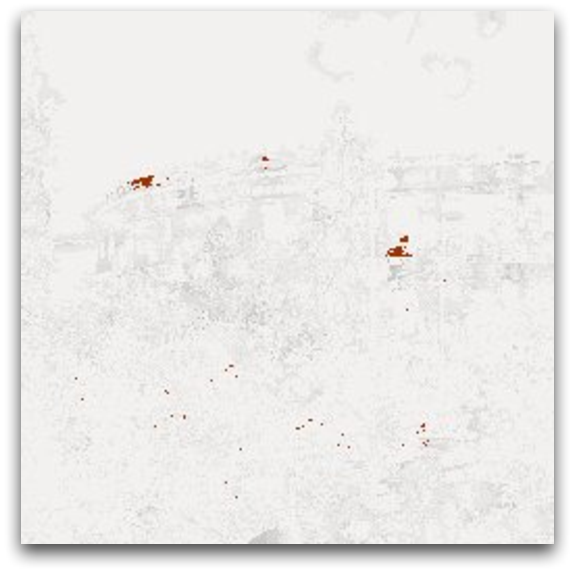
\includegraphics[width=0.33\textwidth]{gfx/itr_limitcycle0}\label{fig:lc0}}%
\subfloat[Period-4 Limitcycle]{%
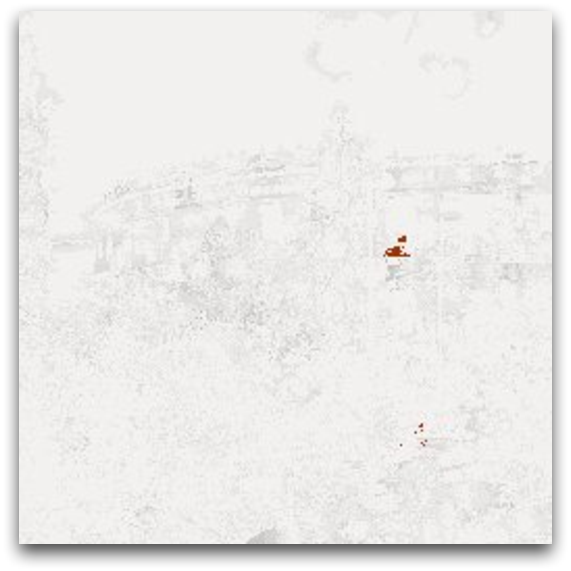
\includegraphics[width=0.33\textwidth]{gfx/itr_limitcycle4}\label{fig:lc4}}%
\subfloat[Period-8 Limitcycle]{%
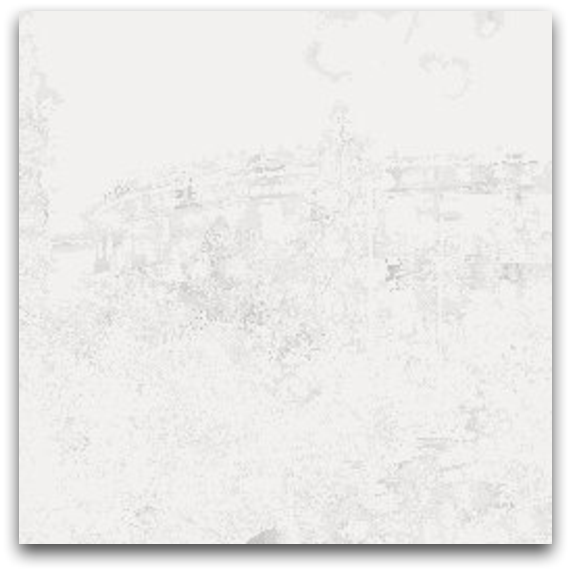
\includegraphics[width=0.33\textwidth]{gfx/itr_limitcycle8}\label{fig:lc8}}%

\caption{Effect of limitcycle detection on iteration count}
\label{fig:limitcycle}
\end{figure}


\begin{figure}[ht]
\centering
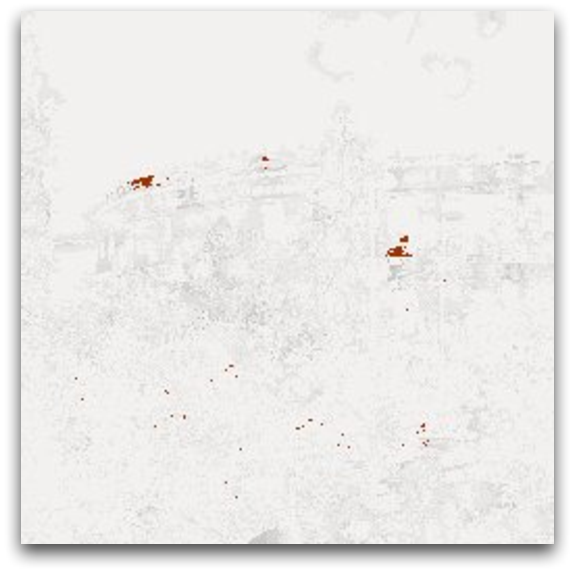
\includegraphics[width=0.6\textwidth]{gfx/itr_limitcycle0.pdf}
\caption{Visualization of Iteration Count}
\label{fig:vis_iteration_count}
\end{figure}



\subsubsection{Limit Cycle, Iterating Dynamical Systems} % (fold)
\label{ssub:limit_cycle_iterating_dynamical_systems}
bla bla  limit cycle attractors...


examining $i = 15762$ shows that the iteration is a period-2 limit cycle.

Implementing a simple period-4 limit cycle detection yields to a speedup of
\fpAdd{\timecuda}{0,0}{99}
\fpDiv{\speedup}{\timegold}{\timecuda}
\begin{equation*}\label{eq:speedup9}
	S = \timegold\ ms/\timecuda\ ms = \speedup
\end{equation*}

Implementing a simple period-8 limit cycle detection yields to a speedup of
\fpAdd{\timecuda}{0,0}{87}
\fpDiv{\speedup}{\timegold}{\timecuda}
\begin{equation*}\label{eq:speedup10}
	S = \timegold\ ms/\timecuda\ ms = \speedup
\end{equation*}


\section{Unrolling Loops and Multiplications} % (fold)
\label{sec:unrolling_loops_and_multiplications}

After unrolling the multiplications 
\fpAdd{\timecuda}{0,0}{83}
\fpDiv{\speedup}{\timegold}{\timecuda}
\begin{equation*}\label{eq:speedup11}
	S = \timegold\ ms/\timecuda\ ms = \speedup
\end{equation*}

\section{Extra luv to rgb Kernel}

After a lot of optimization the most computational task became really small. Now
small function which where a tiny fraction of the complete run time became 
significant. 
After implementing a $luvtorgb$ kernel the speedup is 
\fpAdd{\timecuda}{0,0}{75}
\fpDiv{\speedup}{\timegold}{\timecuda}
\begin{equation*}\label{eq:speedup12}
	S = \timegold\ ms/\timecuda\ ms = \speedup
\end{equation*}



After a lot of optimization the most computational task became really small. Now
small function which where a tiny fraction of the complete run time became 
significant. 




